	L'organisation du groupe Sopra Steria est articulée autour de différentes structures opérationnelles et fonctionnelles donc une structure permanente globale décrite sur la figure \ref{sopraSteriaOrganisation}.

\begin{figure}[h]
	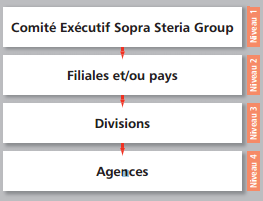
\includegraphics[scale=0.8]{images/entreprise/sopraSteriaOrganisation.png}
	\centering
	\caption{Organisation du groupe}
	\label{sopraSteriaOrganisation}
\end{figure}
		
\subsubsection{Comité exécutif}

	Le comité exécutif est composé du directeur général ainsi que de l'ensemble des directeurs adjoints et est en charge de piloter les projets et affaires les plus importantes du groupe. Il gère aussi l'organisation de la société dans son ensemble.

\subsubsection{Filiales et/ou pays}

	Cette section désigne l'ensemble des grandes entités qui représente soit une partie métier dont nous avons parlé plus haut (conseil, BPS, etc...) soit une zone géographique pouvant faire référence à un pays complet. Ces parties sont alors ensuite découpées en un ensemble de divisions.

\subsubsection{Divisions}

	Les divisions sont créées en fonction de la géographie ainsi que du secteur économique concerné (bancaire, transport, tertiaire etc...).

\subsubsection{Agences}

	Enfin, les divisions sont constituées d'agences qui agissent de manière autonome concernant la gestion de leur budget, des ressources humaines ou encore du pilotage des projets. Dans mon cas, j'ai été assigné à l'agence 512 de la division Banque et Finance de Sopra Steria France. Ainsi, les missions sur lesquelles j'ai été assigné étaient cohérentes avec la division dont je dépendais et concernaient toutes deux des clients banque privée dont je vais parler plus en détails dans la partie suivante.